\section{Physical state}

\begin{frame}{Physical state}
\centering
\hspace{-1cm}
\begin{tikzpicture}[scale=1.15]
	\def\hist{2}
	\def\histx{1}
	\def\model{3}
	\def\priv{2.8}

	\only<1->{
		\draw[step=1cm, gray] (0, 0) grid ++(\hist + \model + \priv, 1) ;
		\draw[decorate, decoration={brace, amplitude=5pt}] (-0.2, 0) -- ++(0, 1) node [midway, xshift=-7mm] {data} ;
	}

	\only<2->{
		\draw[very thick] (\hist, 0) -- ++(0, 1) node[label=above:front] {} ;
	}

	\only<4->{
		\draw[very thick] (\hist + \model, 0) -- ++(0, 1) node[label=above:back] {} ;
	}

	\only<5->{
		\fill[red, opacity=0.2] (\hist + \model, 0) rectangle ++(\priv, 1) ;
		\draw[decorate, decoration={brace, amplitude=5pt}] (\hist + \model + \priv, -0.2) -- ++(- \priv, 0) node [midway, yshift=-5mm] {priv} ;
	}

	\only<6->{
		\fill[green, opacity=0.2] (\hist, 0) rectangle ++(\model, 1) ;
		\draw[decorate, decoration={brace, amplitude=5pt}] (\hist + \model, -0.2) -- ++(- \model, 0) node [midway, yshift=-5mm] {model} ;
	}
	\only<7->{
		\fill[blue, opacity=0.2] (0, 0) rectangle ++(\hist, 1) ;
		\draw[decorate, decoration={brace, amplitude=5pt}] (\hist, -0.2) -- ++(- \hist, 0) node [midway, yshift=-5mm] {hist} ;
	}

	\only<9->{
		\fill[blue, opacity=0.2] (\hist, 0) rectangle ++(\histx, 1) ;
		\draw[decorate, decoration={brace, amplitude=5pt}] (\hist + \histx, - 1) -- ++(- \hist - \histx, 0) node [midway, yshift=-5mm] {hist\textsubscript{+}} ;
	}

	\only<10->{
		\draw[thick, ->, blue] (\hist, 0.5) -- ++(1, 0) node[midway, below] {\footnotesize\texttt{steal}} ;
		\draw[thick, ->, teal] (\hist + \model, 0.5) -- ++(- 1, 0) node[midway, below] {\footnotesize\texttt{pop}} ;
		\draw[thick, ->, red] (\hist + \model, 0.5) -- ++(1, 0) node[midway, below] {\footnotesize\texttt{push}} ;
	}
\end{tikzpicture}
\vfill
\begin{itemize}
	\item[data:]<1-> infinite array storing all values
	\item[front:]<2-> \emph{monotone} index for thieves' end
	\item[back:]<4-> index for owner's end
\end{itemize}
\begin{itemize}
	\item[priv:]<5-> list of private values (controlled by owner)
	\item[model:]<6-> list of contained values
	\item[hist:]<7-> \emph{monotone} list of history values
	\item[hist\textsubscript{+}:]<9-> \emph{monotone} list of extended history values
\end{itemize}
\begin{overbox}<3>
	\begin{mathpar}
		\inferrule*[lab=ChaselevFrontLbGet]
			{
				\iGhost{\gamma\mathrm{.front}}{\iAuth{\textcolor{blue}{front}}}
			}{
				\iGhost{\gamma\mathrm{.front}}{\iFrag{\textcolor{blue}{front}}}
			}
		\and
		\inferrule*[lab=ChaselevFrontValid]
			{
				\iGhost{\gamma\mathrm{.front}}{\iAuth{\textcolor{blue}{front_1}}}
			\and
				\iGhost{\gamma\mathrm{.front}}{\iFrag{\textcolor{red}{front_2}}}
			}{
				\textcolor{red}{front_2} \leq \textcolor{blue}{front_1}
			}
		\and
		\inferrule*[lab=ChaselevFrontUpdate]
			{
				\textcolor{blue}{front} \leq \textcolor{red}{front'}
			\and
				\iGhost{\gamma\mathrm{.front}}{\iAuth{\textcolor{blue}{front}}}
			}{
				\iGhost{\gamma\mathrm{.front}}{\iAuth{\textcolor{red}{front'}}}
			}
	\end{mathpar}
\end{overbox}
\begin{overbox}<8>
	\begin{mathpar}
		\inferrule*[lab=ChaselevHistLbGet]
			{
				\iGhost{\gamma\mathrm{.hist}}{\iAuth{\textcolor{blue}{hist}}}
			}{
				\iGhost{\gamma\mathrm{.hist}}{\iFrag{\textcolor{blue}{hist}}}
			}
		\and
		\inferrule*[lab=ChaselevHistValid]
			{
				\iGhost{\gamma\mathrm{.hist}}{\iAuth{\textcolor{blue}{hist_1}}}
			\and
				\iGhost{\gamma\mathrm{.hist}}{\iFrag{\textcolor{red}{hist_2}}}
			}{
				\textcolor{red}{hist_2} \sqsubseteq_\mathrm{prefix} \textcolor{blue}{hist_1}
			}
		\and
		\inferrule*[lab=ChaselevHistUpdate]
			{
				\iGhost{\gamma\mathrm{.hist}}{\iAuth{\textcolor{blue}{hist}}}
			}{
				\iGhost{\gamma\mathrm{.hist}}{\iAuth{(\textcolor{blue}{hist} \mdoubleplus [v])}}
			}
	\end{mathpar}
\end{overbox}
\end{frame}
